\documentclass{article}
\usepackage[utf8]{inputenc}
\usepackage{multicol}
\usepackage{geometry}
\usepackage{multirow}
\usepackage{booktabs}
\setlength{\columnsep}{30pt} 
\usepackage{frontespizio}
\usepackage[T1]{fontenc}
\usepackage[utf8]{inputenc}
\usepackage{amsfonts}
\usepackage{amsmath}
\usepackage{bm}
\usepackage{empheq}
\usepackage{csquotes}
\usepackage[backend=biber,sorting=none]{biblatex} 
\usepackage{lipsum}
\usepackage{listings}
\usepackage[font=small,labelfont=bf]{caption}
\usepackage{url}
\usepackage[table]{xcolor}
\usepackage{float}
\usepackage[section]{placeins}
\graphicspath{ {./Figures/} }
\usepackage{graphicx,subfig,caption}
\usepackage{subfig}

\usepackage{algorithm,algorithmic}

\addbibresource{bibliography.bib}  

\usepackage{nicematrix}
\definecolor{codegreen}{rgb}{0,0.6,0}
\definecolor{codegray}{rgb}{0.5,0.5,0.5}
\definecolor{codepurple}{rgb}{0.58,0,0.82}
\definecolor{backcolour}{rgb}{0.95,0.95,0.92}







\geometry{margin=2cm}

\lstdefinestyle{mystyle}{
	backgroundcolor=\color{backcolour},
	commentstyle=\color{codegreen},
	keywordstyle=\color{magenta},
	numberstyle=\tiny\color{codegray},
	stringstyle=\color{codepurple},
	basicstyle=\ttfamily\footnotesize,
	breakatwhitespace=true,
	breaklines=true,
	captionpos=b,
	keepspaces=true,
	numbers=left,
	numbersep=8pt,
	showspaces=false,
	showstringspaces=false,
	showtabs=false,
	tabsize=2,
	breakindent=0pt ,
	columns=fullflexible,
	postbreak=\mbox{\textcolor{red}{$\hookrightarrow$}\space}
}



\lstset{breaklines=true}


\begin{document}
	
	
\title{Adaptive threshold for anomaly detection in vital parameters}
\author{R. Lorusso}
\date{2023 - University of Bari Aldo Moro}
	
\maketitle
	
\begin{multicols*}{2}
		
\section*{Abstract}
\begin{it}
%The aim of this work is to provide a model for effectively identify anomalies in vital parameters time series selected from VitalDB dataset \cite{VitalDB}. The employed model is an LSTM autoencoder as a tool to identify anomalies in such temporal data by the evaluation of the mean reconstruction error.
%Furthermore an adaptive threshold selection based on the training data reconstruction error is proposed, with the aim of improving the explainability of the model without relying on an arbitrary threshold.

The aim of this work is to provide an algorithm for the adaptive threshold selection starting by the training data reconstruction error, to effectively identify anomalies in vital parameters time series selected from VitalDB dataset \cite{VitalDB}. This could result in the improvement of explainability in evaluation methods based on the reconstruction error. The employed model is an LSTM autoencoder. 
\end{it}
		
		
		
\section{Introduction}
		
The detection of anomalies, also known as outliers, is an integral practice across a diverse range of disciplines. Anomalies can indicate a breach of a system or network, signal abnormal physiological levels, or even flag the occurrence of fraud. Regardless of the particular application, analytics and machine learning models have the potential to provide both predictive and descriptive value. Anomaly detection can be used to inform about anomalous data that can be indicative of health complications. This kind of information can be very useful to professionals as a first insight into a possible patient problem. Since providing care and tracking patient vitals signals can be hard to maintain over time, machine learning can be very helpful by automatically detecting rare deviations from normal data trends, thus providing health care professionals with useful information with which to make more accurate and quicker clinical decisions. However, what is to be considered an anomaly is never clearly defined. The main assumptions are that anomalies are frequent and somehow differ from normal data. Frustrating anomalies can differ substantially from each other, thus introducing more uncertainty about their nature. Sometimes oscillations in the test data can be detected as anomalies, introducing false alarms. Especially in the e-health domain, we are interested in reducing or minimizing the number of false alerts, since a high false alarm rate can decrease trust in the system and in the alarm itself. In order to cope with these problems, an adaptive threshold selection based on the mean reconstruction error on training data is proposed.
In section \ref{model}, we’ll start with a formal definition of a general autoencoder and how it can be employed to identify anomalies. Section \ref{dataset} describes the dataset and its selected features through a preliminary exploratory data analysis. Then we can move on to Section \ref{preprocessing}, focusing our attention on the features and preprocessing strategy. Finally, in Section \ref{model_development} , it introduces the model implementation, which is further evaluated in Section  \ref{results}  by means of the obtained results.
		


\section{Employed model}
		\label{model}
Autoencoders are widely used for anomaly detection tasks in a variety of different fields and for many purposes. The choice of an LSTM autoencoder is motivated by the use of time series in the health domain \cite{VitalDB}. An autoencoder is a feed-forward neural network used to learn a latent representation of unlabeled input data, and it is trained to reconstruct the input at the output layer.. Autoencoders are made by an encoder and a decoder, which can be described by two maps $\Phi$  and $\Psi$ on $X \in \Re^n$, $Y \in \Re^d$, $d < n$ such as:
\begin{align*}
			\Phi : X \rightarrow  Y \\
			\Psi : Y \rightarrow  X  
\end{align*}
for which the goal is to minimize the mean squared error between the input and the output layer
\begin{equation*}
			argmin_{\Phi,\Psi}|| X -  (\Psi  o \Phi) X ||^2.
\end{equation*}
The main assumption is that the data fed to the model in the training phase is to be considered normal. Since the neural network encodes an input data point in a latent space learned from normal data and decodes it from the very same space to reconstruct its original form, we can evaluate the degree of fitness of the model by measuring the reconstruction error through a distance metric. If the reconstruction error is large enough, then we can assume that the tested sample can be considered an anomaly since it doesn't fit the latent space and is different from the training data.

	
\section{Dataset Description}
	\label{dataset}
The dataset employed is called VitalDB \cite{VitalDB}, it contains high-resolution multi-parameter data from 6,388 surgical patients. The mean age of the patient is 57 years. Among the plethora of different features, the following have been selected:
\begin{itemize}
	\setlength\itemsep{-0.1em}
			\item Diastolic blood pressure (DBP). Unit: mmHg;
			\item Systolic blood pressure (SBP). Unit: mmHg;
			\item Body temperature (BT). Unit: C°;
			\item Heart rate (HR). Unit: beats/minute;
			\item Respiratory rate (RR). Unit: breaths/minute;
\end{itemize}
which are the basic vital parameters useful for a first assessment of a patient's health state. Since the dataset contains records of surgical patients vital parameters, the ones with the healthiest values have been selected by means of the ASA physical status system  \cite{ASA}. Only those records with an ASA grade lower than three are retained for training the model, resulting in the distribution depicted in the figure. A percentage of this data is held out for testing and evaluating the model, which will be used further for detecting anomalies on the portion of the dataset with an ASA equal to three, i.e. "patients with severe systemic disease". From Fig. \ref{fig:raw_data}, it's possible to observe how the distribution of such data is more irregular and slightly shifted to the right side of the chart for the first three parameters, while the distribution of respiratory rate and body temperature values is very similar.

\begin{figure}[H]
			\centering
			\subfloat[ASA  <  3]{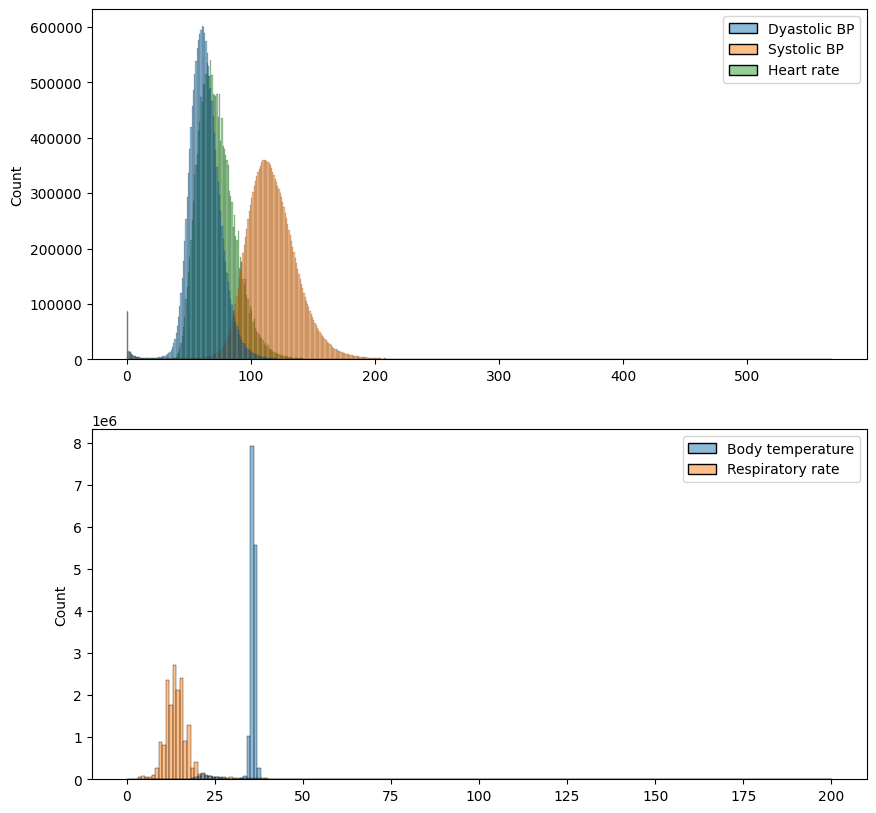
\includegraphics[width=0.5\linewidth]{imgs/raw_data.png}\label{fig:raw_data}}
			\subfloat[ASA == 3]{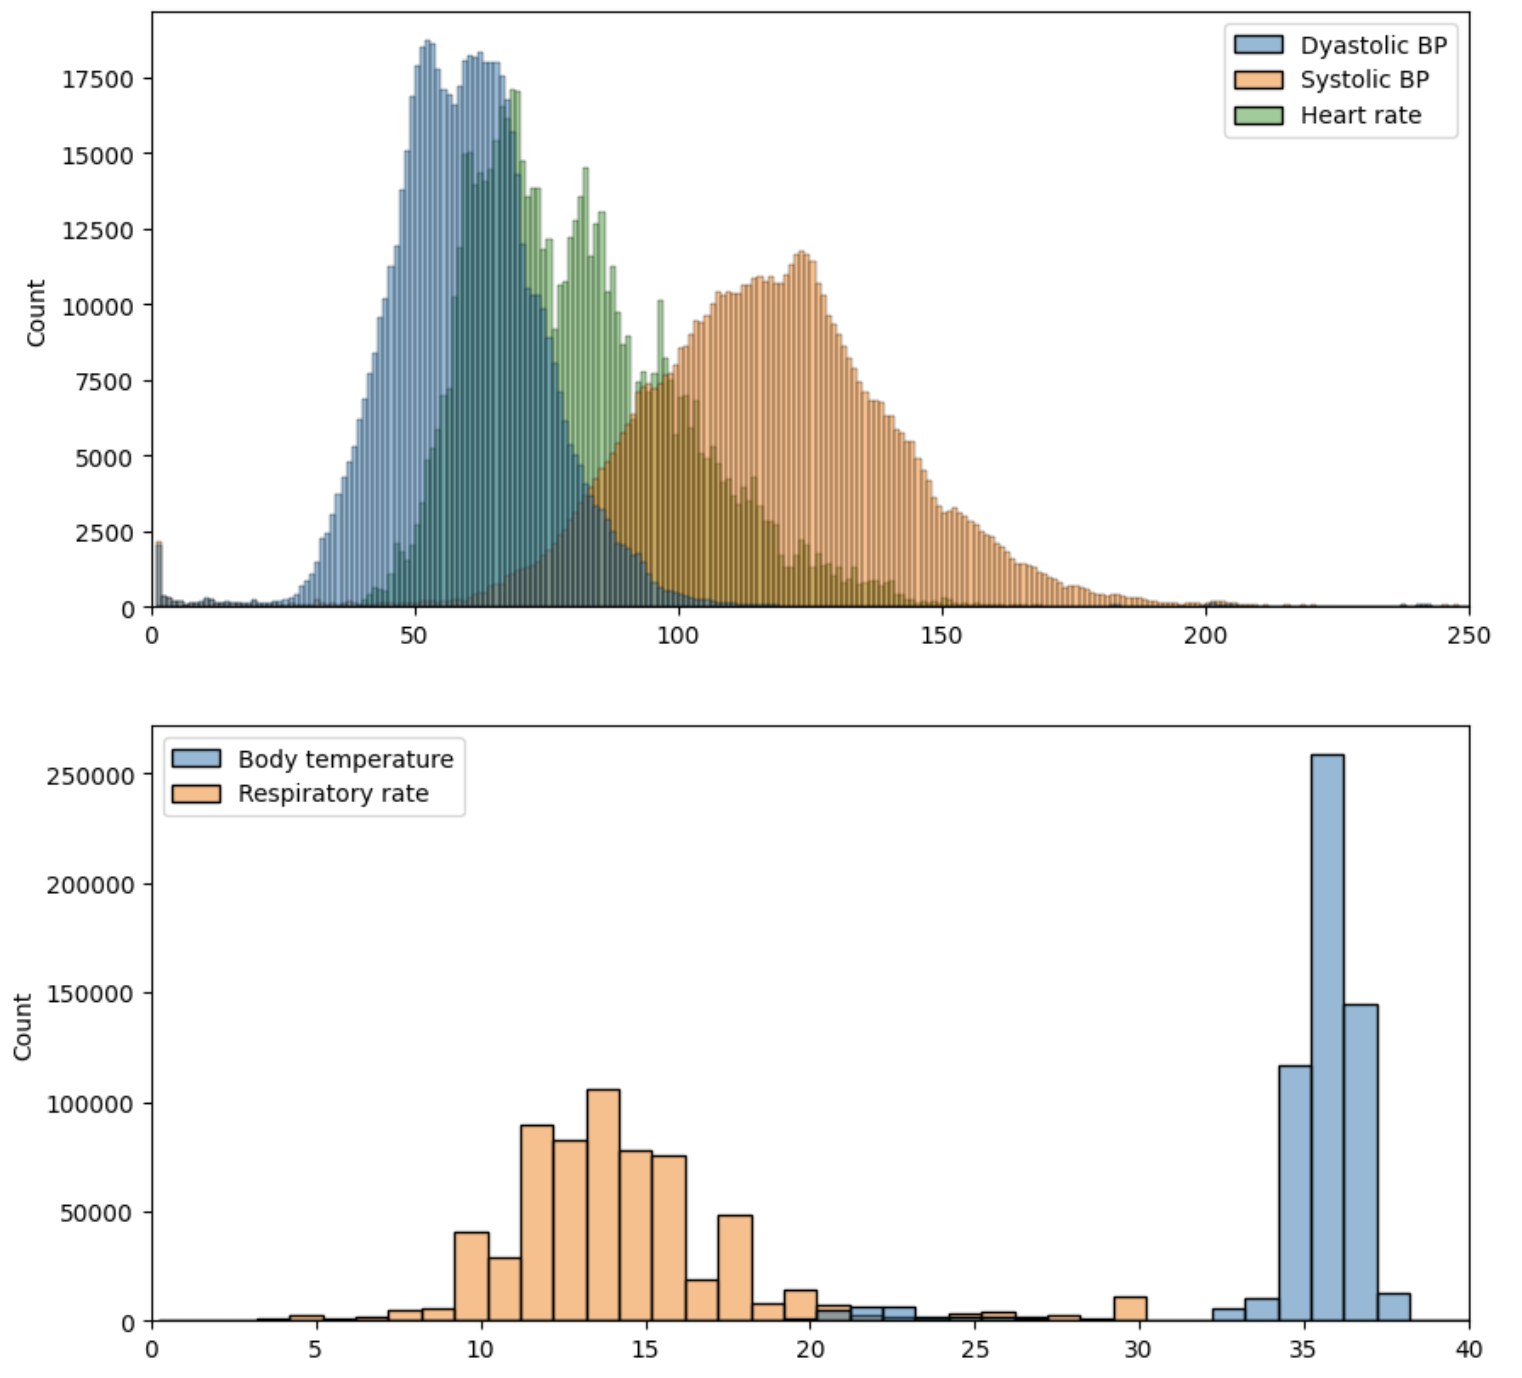
\includegraphics[width=0.5\linewidth]{imgs/asa_eq_3.png}\label{fig:raw_data1}}
			\caption{Data distribution}
\end{figure}
Since every feature presents anomalous values, the following section describes the preprocessing strategy applied to retain only the feature values that can be considered normal.
Before going into details of the preprocessing strategy, it's worth noting that the data has been collected from surgical patients during the perioperative period \cite{VitalDB}. Considering this context, it is possible to deduce that the results obtained by a model trained on such data could be useful in the same kind of context but may be wrong in another one, such as during physical activity. We will talk about this in the section \ref{ethics} related to the ethical implications.

\section{Feature Engineering}
		\label{preprocessing}
As anticipated, it has been necessary to retain only the values that can be considered healthy. This is done by following both common knowledge, as in the case of body temperature, and internationally approved guidelines as in the case of blood pressure \cite{ESC}.


\subsection{Data cleaning}
Every feature record has been cleaned of NaN and negative values, which were consistently present in the data. Then time series are cleaned from values outside the following ranges:

		\begin{itemize}
				\setlength\itemsep{-0.1em}
			\item Diastolic blood pressure: 30-100;
			\item Systolic blood pressure: 85-130;
			\item Body temperature: 35-37.2;
			\item Heart rate: 40-120;
			\item Respiratory rate: 8-22.
		\end{itemize}
These range values are a bit wider than the optimal ones to preserve some variability and noise in the data without making the model too rigid in detecting anomalies. However, restricting the data to a range can introduce sudden changes in time series values, thus negatively affecting its quality. To partially overcome this problem, the values outside a range could be replaced with the mean value of the sample or interpolated for smoothing the gap between two values. After restricting the values in ranges, we obtain a new data distribution depicted in the figure \ref{fig:clean_data}. Wider data intervals will result in looser anomaly detection.
\begin{figure}[H]
			\centering
			\subfloat{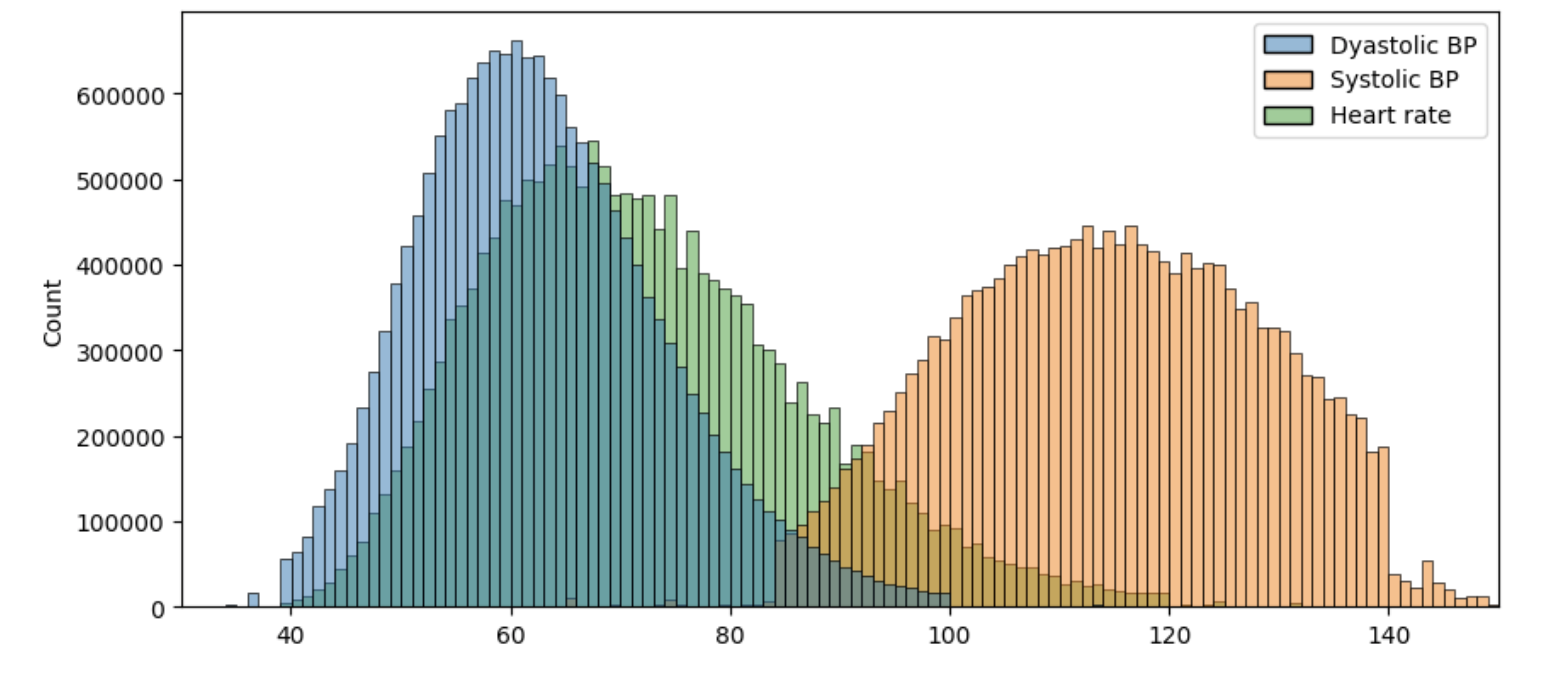
\includegraphics[width=0.5\linewidth]{imgs/clean_data.png}\label{fig:clean_data}}
			\subfloat{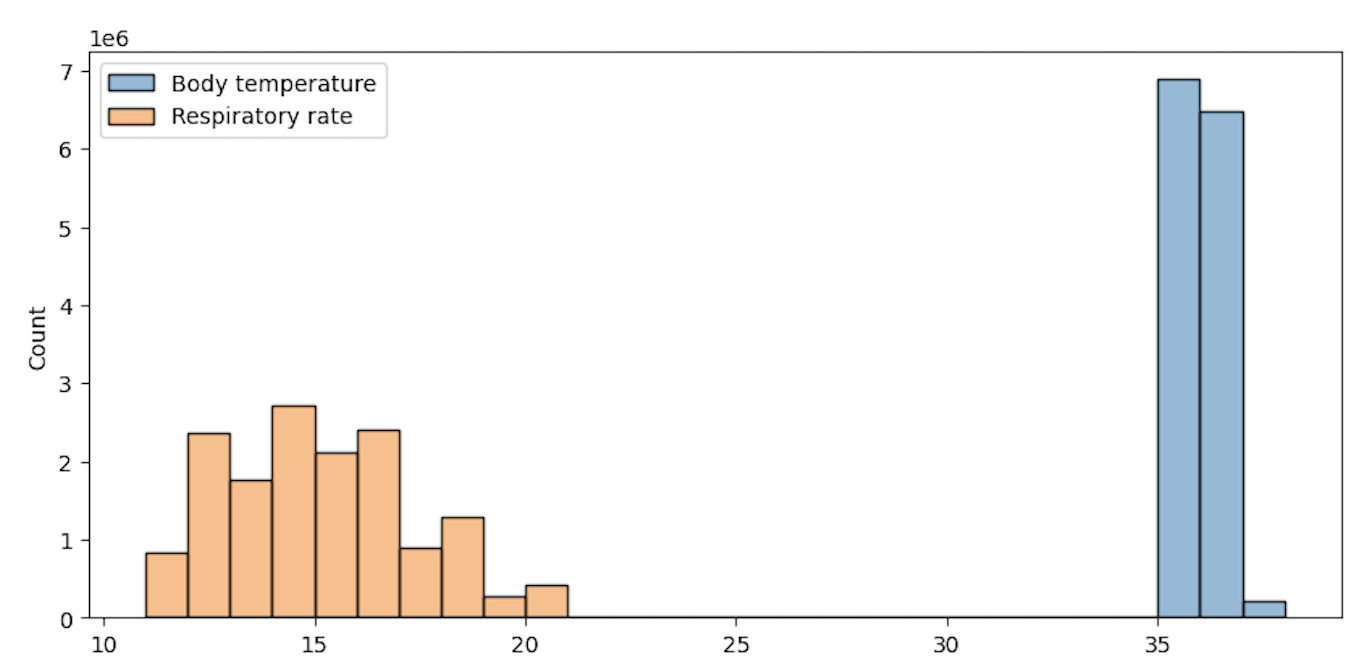
\includegraphics[width=0.5\linewidth]{imgs/bt_rr_clean.png}\label{fig:bt_rr_clean}}
			\caption{Data distribution restricted to ranges}
\end{figure}
As the ultimate step, every record that is either empty or has a negative mean is removed since vital parameters can't have negative values or be null.
Figure 3 shows an example of a diastolic blood pressure sample, before and after it's cleansed.
\begin{figure}[H]
	\centering
	\subfloat[Before cleansing]{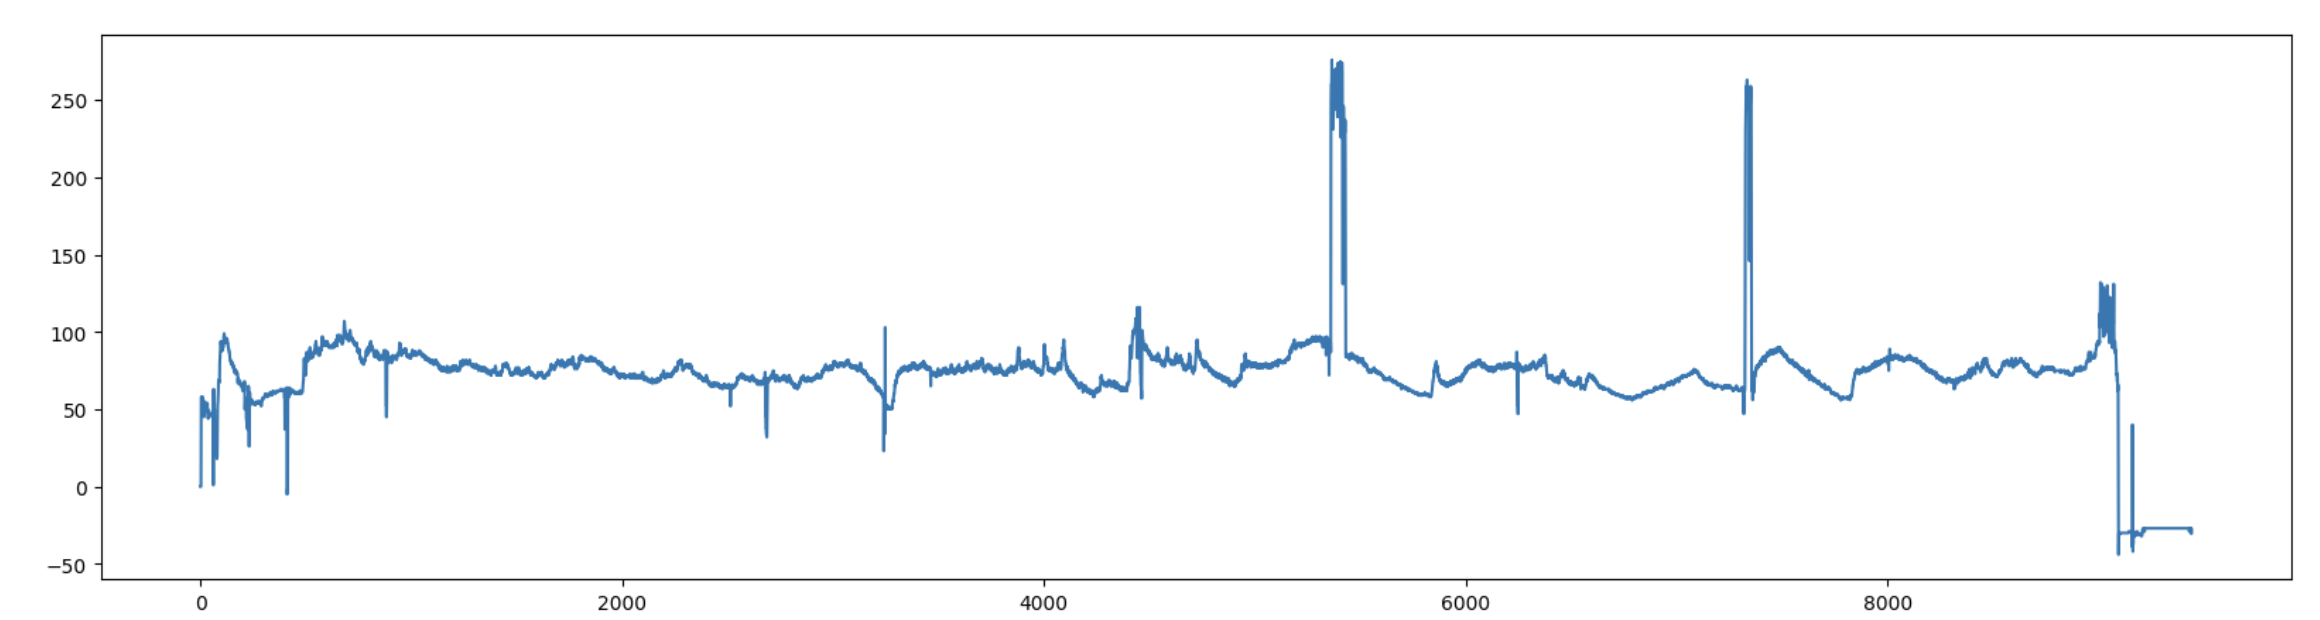
\includegraphics[width=0.9\linewidth]{imgs/before.png}\label{fig:before}}
\end{figure}
\begin{figure}[H]
	\label{fig:after}
	\centering
	\subfloat[After cleansing]{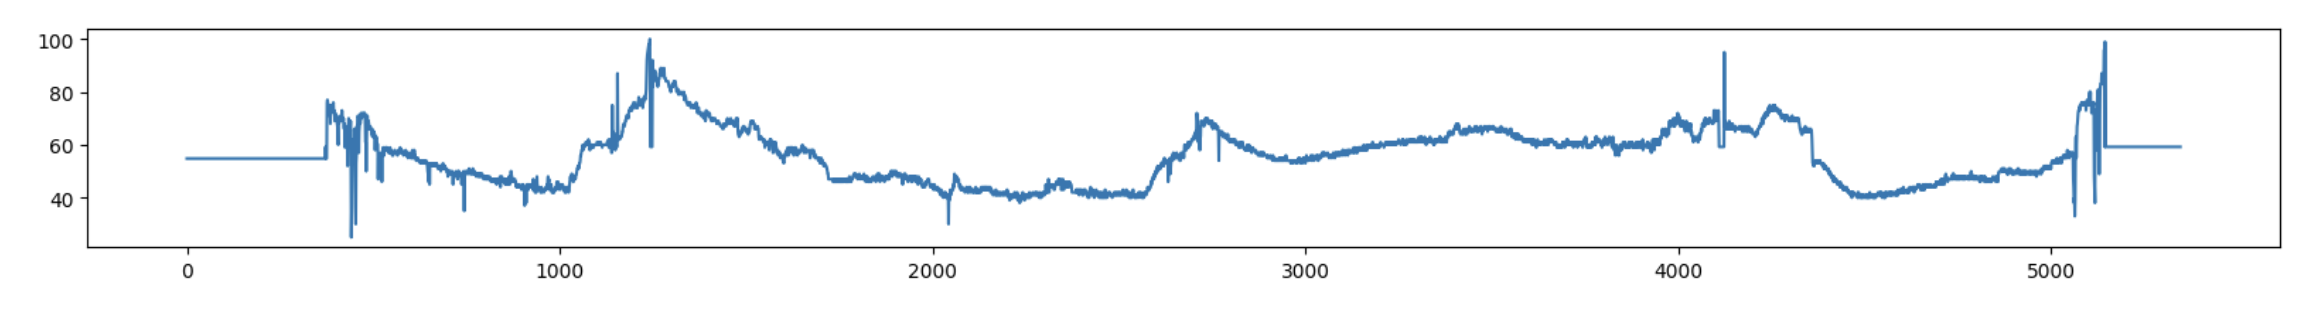
\includegraphics[width=0.99\linewidth]{imgs/after.png}}
	\caption{Diastolic blood pressure sample cleansed from noise and anomalous values}
\end{figure}


\subsection{Data bundling and chunking}
After the data has been cleansed of anomalous values, the time series along the different features are concatenated to create five unique sequences. These are then chunked into ones of equal length to be fed into the model.
This step was necessary because the model expects a uniform sequence length among all the features. Other techniques have been tried, such as padding or truncation, but poor results were obtained.
Since feature values follow a normal distribution, mean-variance normalization has been applied.


\section{Model development}
\label{model_development}
The model employed for this task is a multivariate LSTM autoencoder, and the choice is motivated by the time series data. It is implemented using the Keras library.
In figure \ref{fig:model}, the model architecture is depicted. As we can see from the input shape, the time series length is equal to 4678. This value can be diminished or enlarged to carry out a more local or global analysis, respectively. In this case, the input shape is selected as the minimum length of the records across the different features.
	


\begin{figure}[H]
	\centering
	\subfloat{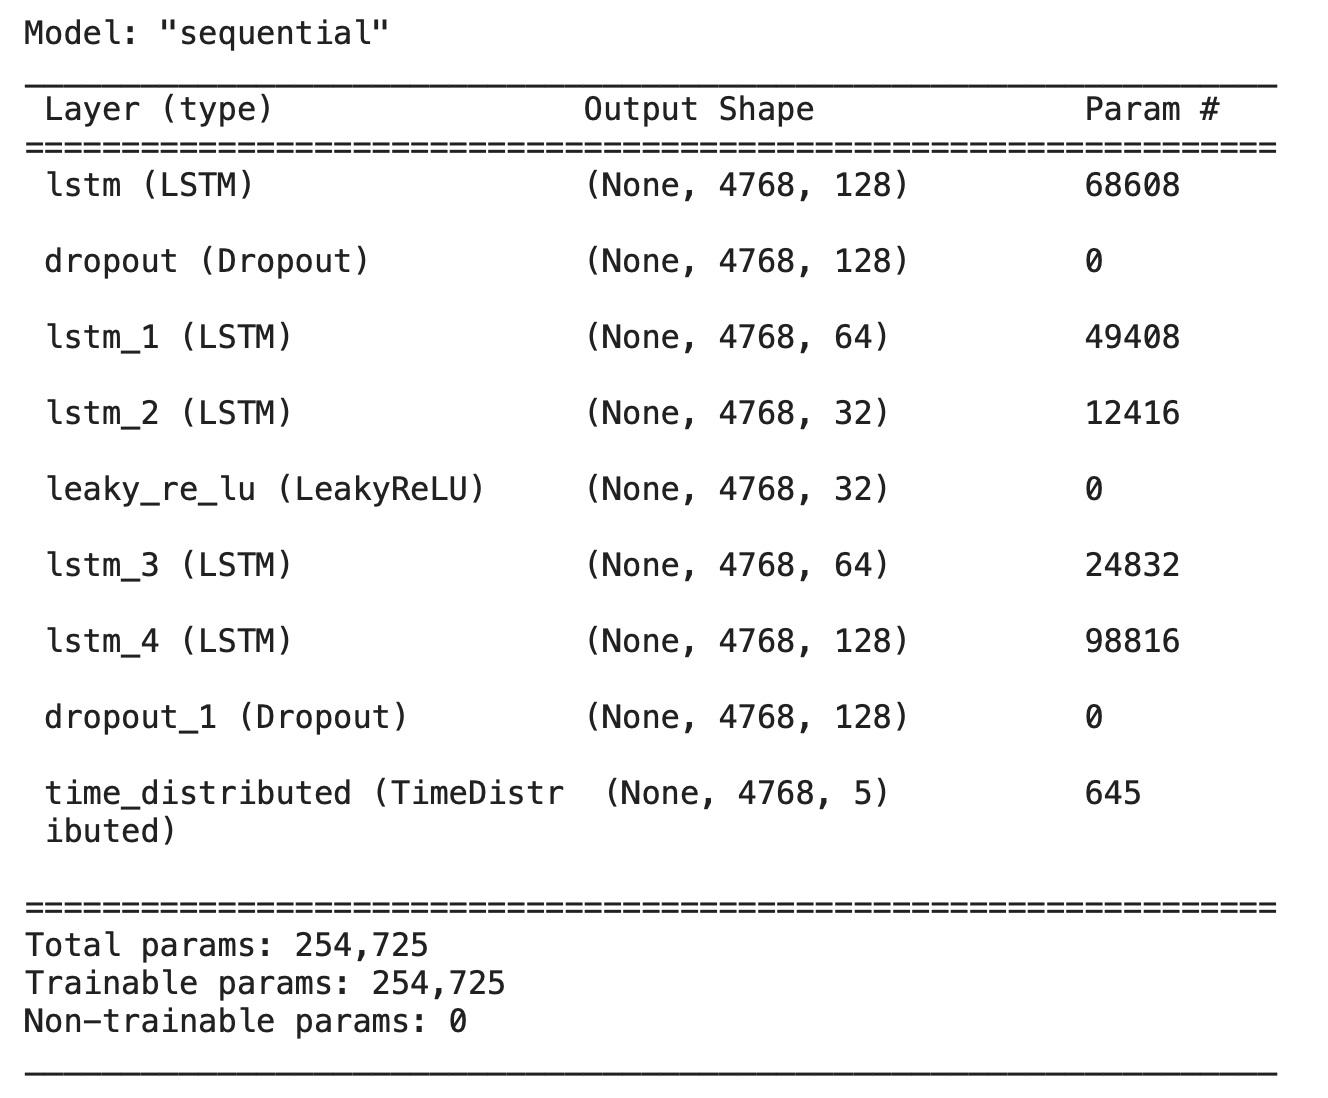
\includegraphics[width=0.99\linewidth]{imgs/model.png}}
	\caption{LSTM autoencoder architecture}
	\label{fig:model}
\end{figure}

\subsection{Configuration} 
The final configuration of the parameters has been obtained after several training sessions.
The best results are yielded with the following parameter settings: 
\begin{itemize}
		\setlength\itemsep{-0.1em}
	\item epochs = 50;
	\item loss function =  Mean Squared Error;
	\item bias regularizer = 0.3;
	\item recurrent regularizer = 0.1;
	\item batch\_size = 64;
	\item validation split = 0.1.
\end{itemize}

By the moment that we are in a semi-supervised context since we are selecting the data by means of the ASA parameter, it has been possible to hold out a part of the data in order to evaluate the model performances on such testing data. The 80\% of data with an ASA less than three is retained for training, and the remaining 20\% is held out for testing.
In section \ref{results}, a comparison between the mean reconstruction errors made on the training and testing data is shown in order to see if the model behaves as expected by producing a similar mean reconstruction error for the two sets.
Finally, the model is employed to reconstruct the population data with an ASA of greater than 3, for which a greater reconstruction error is expected.

\section{Adaptive threshold selection}
As already discussed in the introduction, the identification of anomalies relies on the assumption that they are rare and differ from normal data. In the context of autoencoders, an anomaly is detected by evaluating the reconstruction error by means of a threshold whose value is set manually. Most of the time, this value is determined by looking at the distribution of reconstruction errors, although recent studies propose standard deviation-based methods to adapt such a value \cite{adaptivethresh}.
In this section, a simple approach to adapting the threshold is described on the basis of the mean reconstruction error made by the autoencoder on the training data. Given the reconstruction error for the entire training set, it is possible to select the threshold value that encloses a given percentage of data below such a value. Since we are interested in identifying anomalies, we can start with the mean reconstruction error made on the training set and increment it until the above condition is met. As a result, an input sequence will be considered an anomaly if its reconstruction error differs from a given percentage of train data.
A formal definition is given below.

\begin{algorithm}[H]
\caption{Adaptive threshold selection}
\begin{algorithmic}
	\label{threshold}
	\STATE $X$ \COMMENT{Autoencoder input, array of time series}
	\STATE $Y$ \COMMENT{Autoencoder output, array of time series}
	\STATE $n\_samples \gets len(X)$ 
	\STATE $mean\_rec\_err $ \COMMENT{Train set mean reconstruction err}
	\STATE $target \gets 0$
	\STATE $percentage \gets .98$
	\STATE $step \gets 1 - percentage$
	\STATE $factor \gets 1 - step$
	
	\WHILE{target < percentage}
			\STATE $j \gets 0$
				\STATE $factor \gets factor + step$
				
				\FOR{i in  range(0,n\_samples)}
					\STATE $err \gets norm2(X[i] - Y[i])$
					\IF{$err \le mean\_rec\_err \times factor$)}
					\STATE $j \gets j+1$
					\ENDIF
				\ENDFOR
			\STATE$target \gets j \div n\_samples$
	\ENDWHILE\
	
	\STATE $threshold \gets factor \times mean\_rec\_err$
	\RETURN $threshold$
\end{algorithmic}
\end{algorithm}
Convergence is guaranteed by additional constraints, such as the maximum number of iterations, not presented in the formal definition.
As reported in the algorithm comments, $X$ and $Y$ are arrays of time series; since every feature can be represented as an array of time series, the algorithm has to be executed $N$ times, where $N$ is the number of features. By doing so, it is possible to identify anomalies by analyzing the single features, thus enhancing the model's explainability.

			
\section{Experimental results}
\label{results}
In this section are illustrated the results obtained by applying the adaptive threshold selection algorithm on the training data, which will be further used to detect anomalies in testing data by the evaluation of the mean reconstruction error obtained on the features.
Figure \ref{fig:loss} reports the loss obtained after training the model for 50 epochs.
Then the autoencoder is used to perform predictions both on the portion of data held out from the training set and on the data with ASA equal to three. As expected, the reconstruction error of the former is lower than the latter; the results are shown in the table \ref{table:results} for every feature.

\begin{figure}[H]
	\centering
	\subfloat{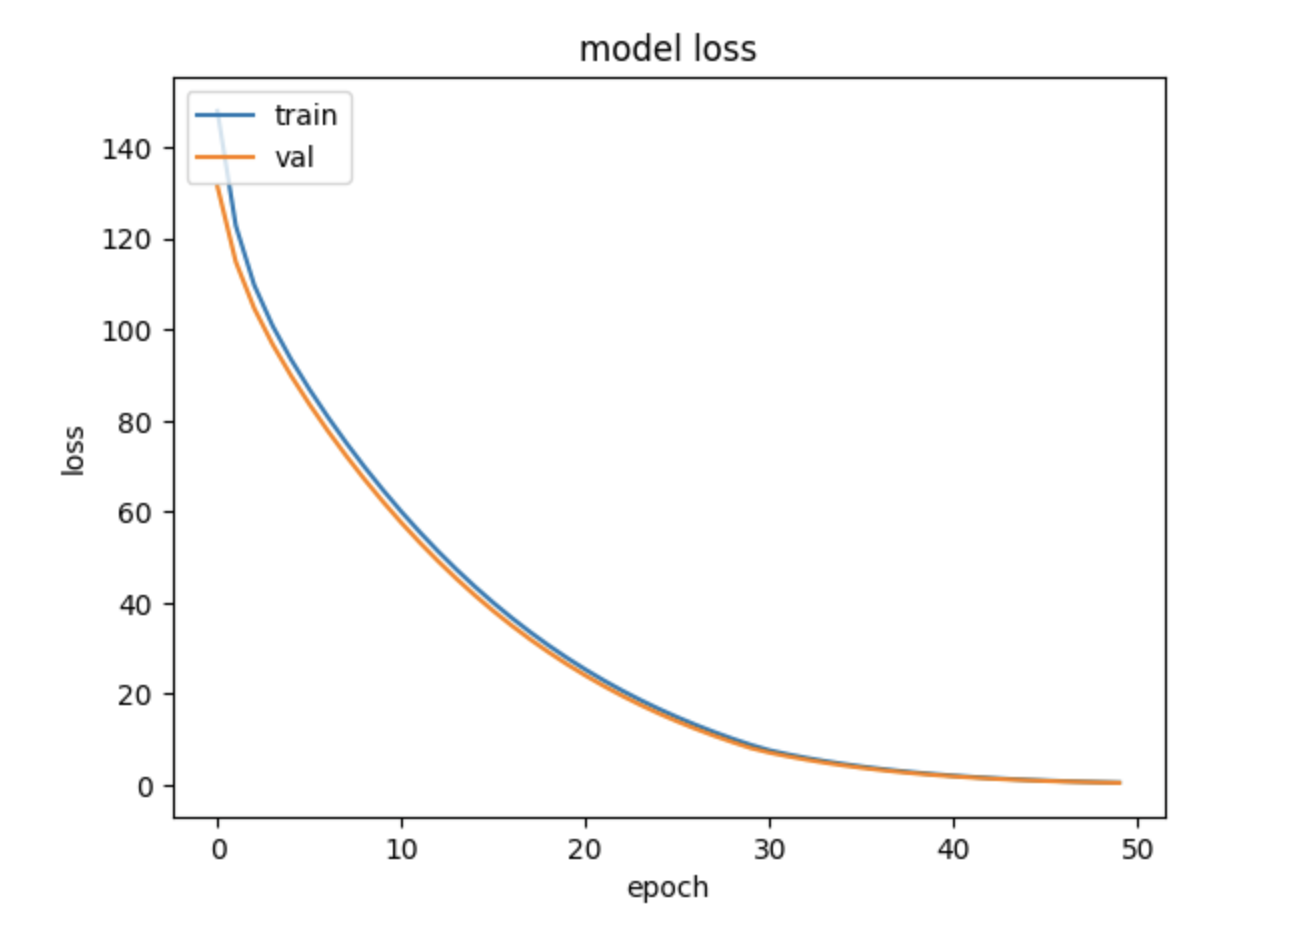
\includegraphics[width=0.8\linewidth]{imgs/loss.png}}
	\caption{Loss function}
	\label{fig:loss}
\end{figure}


\subsection{Threshold selection}


\begin{table}[H]
	\centering
	\begin{tabular}{    p{0.25\linewidth} | c | c | c  } 
		
		Features & Train set  & Test set  &  ASA == 3 \\ 
		\hline\\[-2.7ex]
		DBP & 7.5 & 7.6 & 21.8 \\
		SBP & 6.3 & 6.4 & 16.0 \\
		BT & 3.8  & 3.8 & 15.3 \\
		HR & 5.8 & 5.5 & 10.0 \\
		RR & 4.8 & 4.8 & 15.4 \\
		\hline
		Average & 5.6 & 5.6 & 15.7
	\end{tabular}
	\caption{Features mean reconstruction error}
	\label{table:results}
\end{table}

It is worth noting that the mean reconstruction error of the features is very similar for the training and test sets since they belong to the same population of data, i.e., the data cleansed from anomalous values, whereas the portion of data with ASA == 3 has a significantly greater reconstruction error for all the features.
Starting with the values shown in the column Train Set, execution of \b{Algorithm \ref{threshold}} on the training data returned the following threshold values for features:

\begin{table}[H]
	\centering
	\begin{tabular}{    p{0.5\linewidth} | p{0.3\linewidth} } 
		
		Features & Threshold \\ [0.5ex] 
		\hline
		Diastolic Blood Pressure & 10.9 \\
		Systolic blood pressure & 9.3 \\
		Body Temperature & 6.9 \\
		Heart Rate & 13.6 \\
		Respiratory Rate & 11.9 \\
	\end{tabular}
	\caption{Features threshold}
	\label{table:thresholds}
\end{table}

This values are depicted in the figure \ref{fig:thresholds}. As we can see, the threshold encloses 98\% of mean reconstruction errors, and indeed, the outliers are more sparse and distant from the value distribution.

\begin{figure}[H]
	\centering
	\subfloat{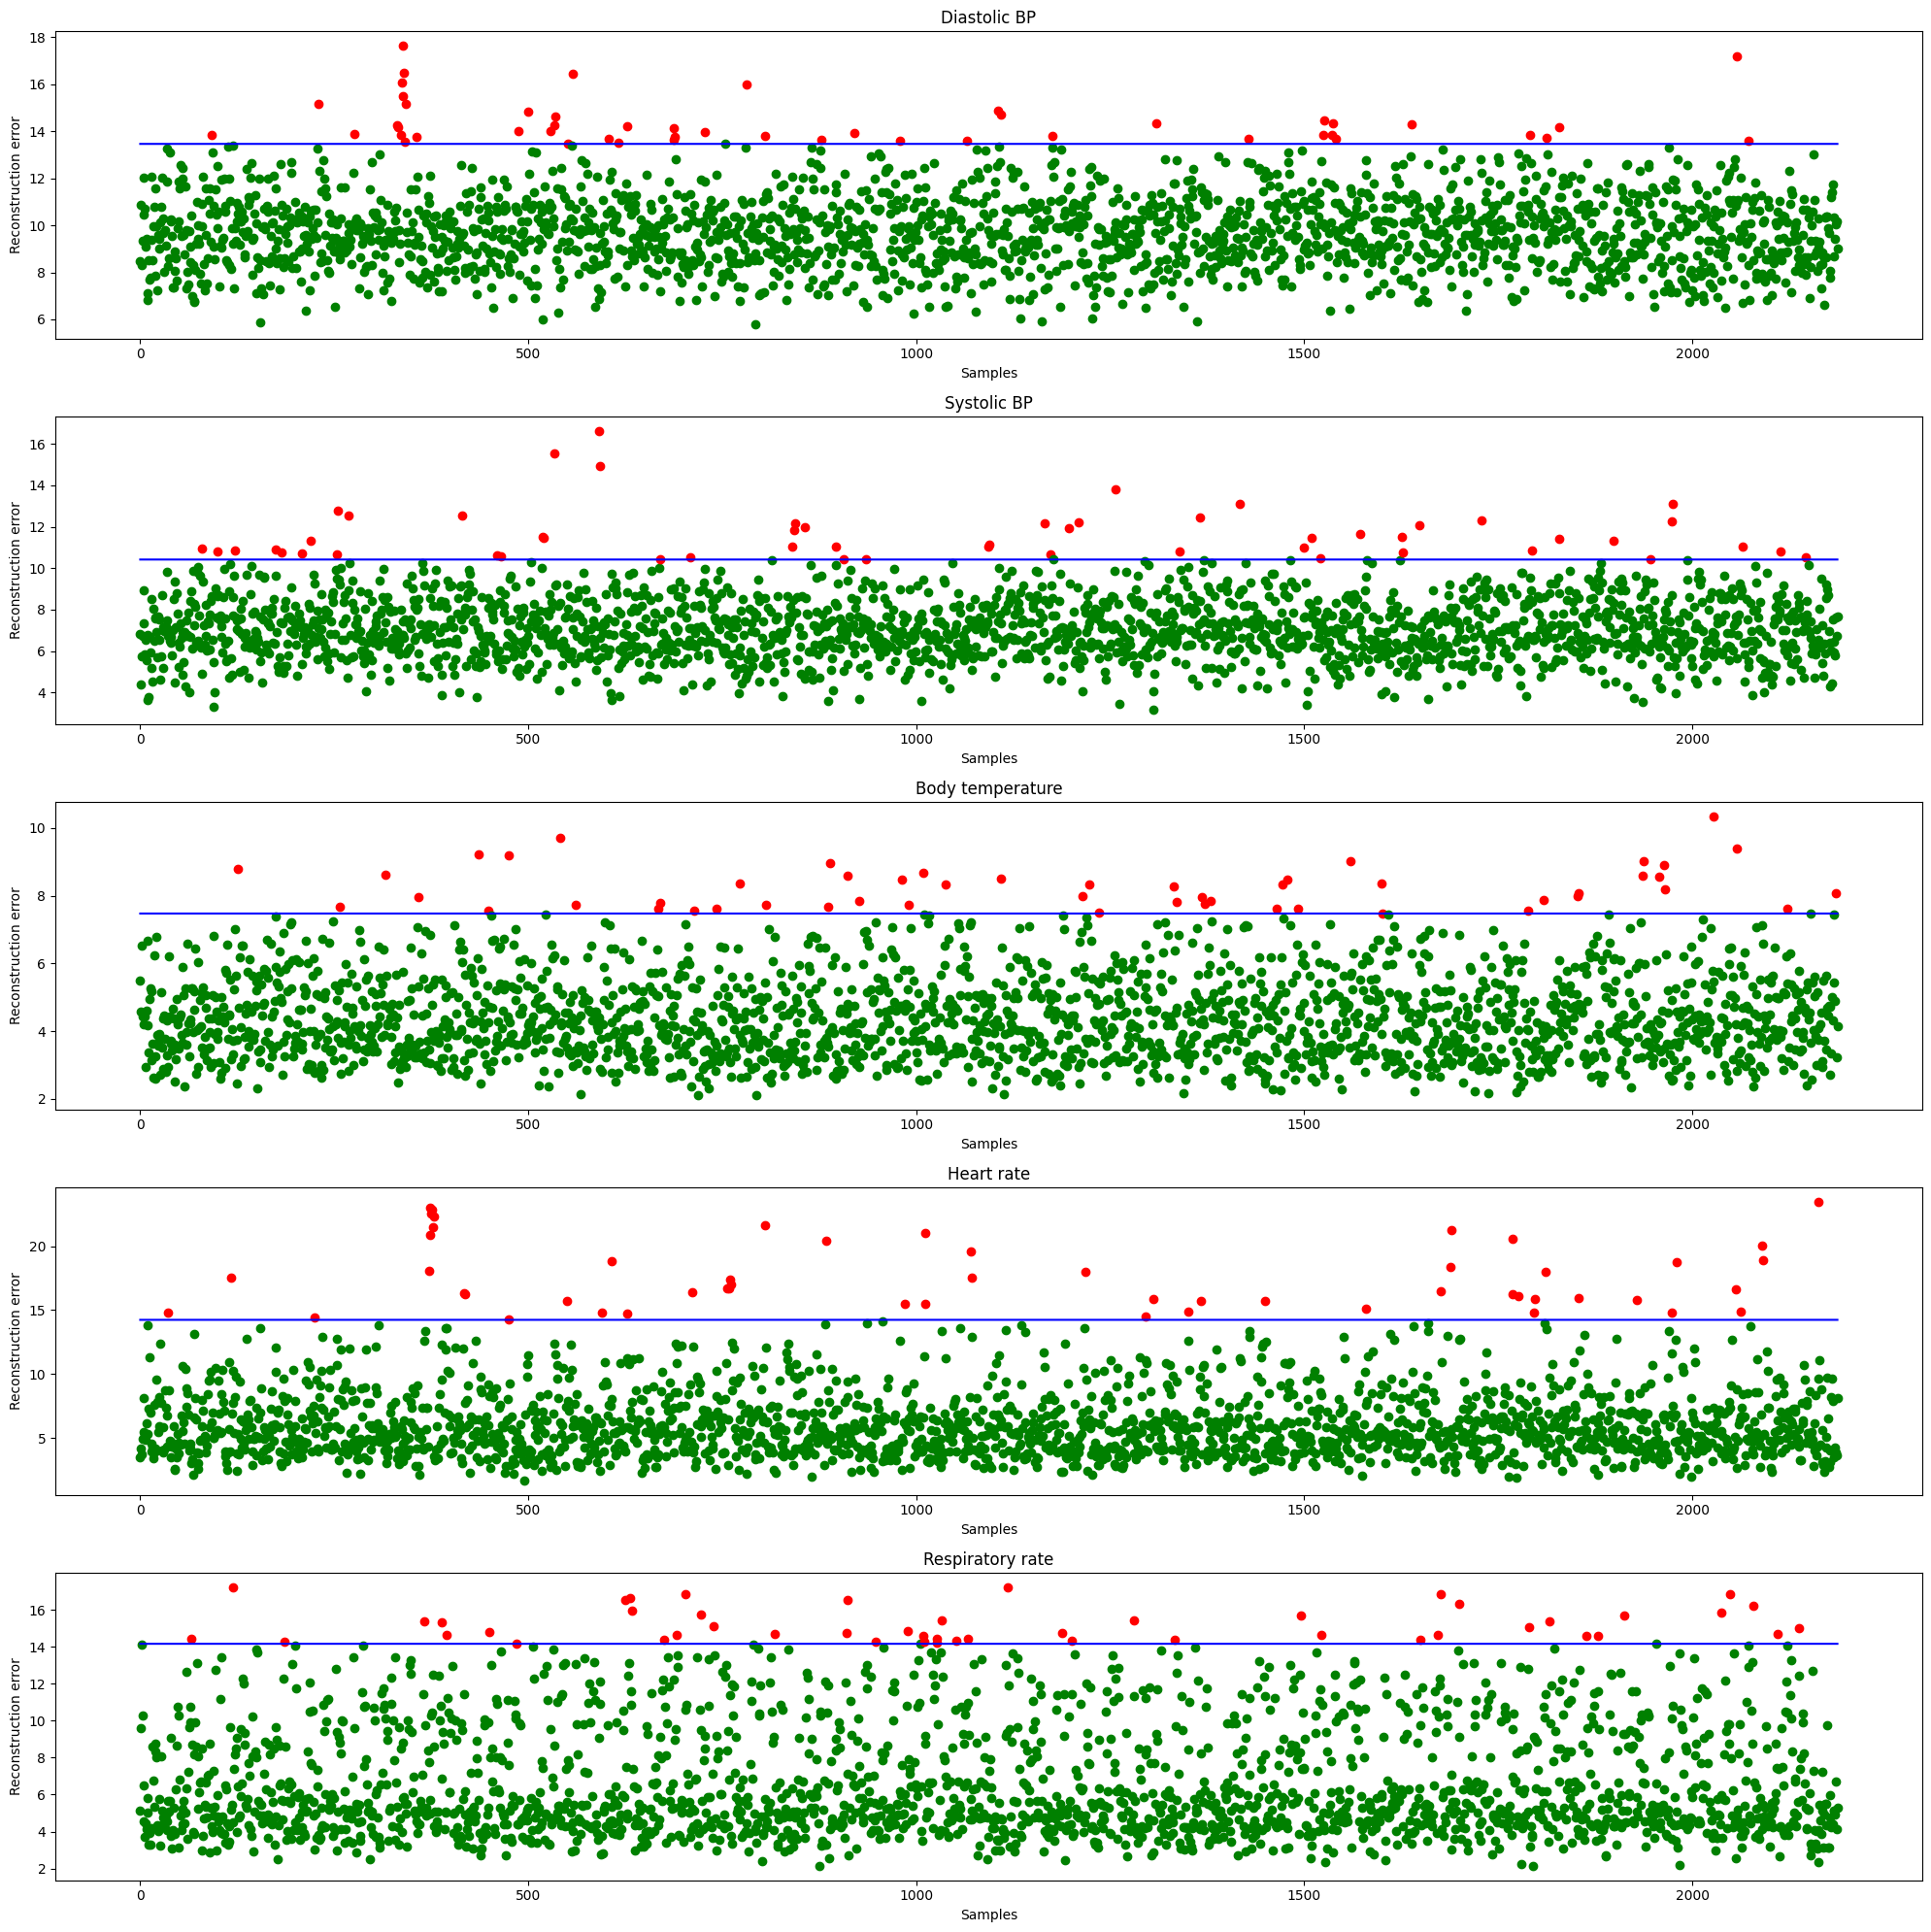
\includegraphics[width=\linewidth]{imgs/feature_train_err_1.png}}
	\caption{Thresholds obtained from training set}
	\label{fig:thresholds}
\end{figure}

\subsection{Anomaly detection on test data}
Now it is possible to use the threshold values presented previously to identify anomalies in testing data. Looking at tables \ref{threshold} and \ref{table:results}, we expect a high anomaly rate on data with an ASA equal to three and a lower one on the held-out data. Table \ref{table:test_results} shows the percentage of anomalies identified in the two groups.
\begin{table}[H]
	\centering
	\begin{tabular}{    p{0.25\linewidth} | c | c | c  } 
		
		Features &  ASA < 3 (test set) &  ASA == 3 \\ 
		\hline
		DBP  & 2\% & 63\% \\
		SBP & 3\% & 57\% \\
		BT & 2\% & 56\% \\
		HR & 2\% & 20\% \\
		RR & 2\% & 19\% \\
		\hline
		Average & 2.2\% & 43\%
	\end{tabular}
	\caption{Percentage of anomalies in tested data}
	\label{table:test_percentage}
\end{table}

As expected, the group with an ASA equal to three has a high anomaly rate since it doesn't fit the autoencoder latent space, while the testing group has exactly the same amount of anomalies as the training set from which it was picked.
Figures \ref{fig:feature_test_data} and \ref{fig:feature_asa3_data} depict the results obtained by applying the thresholds shown in table \ref{table:thresholds} to evaluate reconstruction error on such data.

\begin{figure}[H]
	\centering
	\subfloat{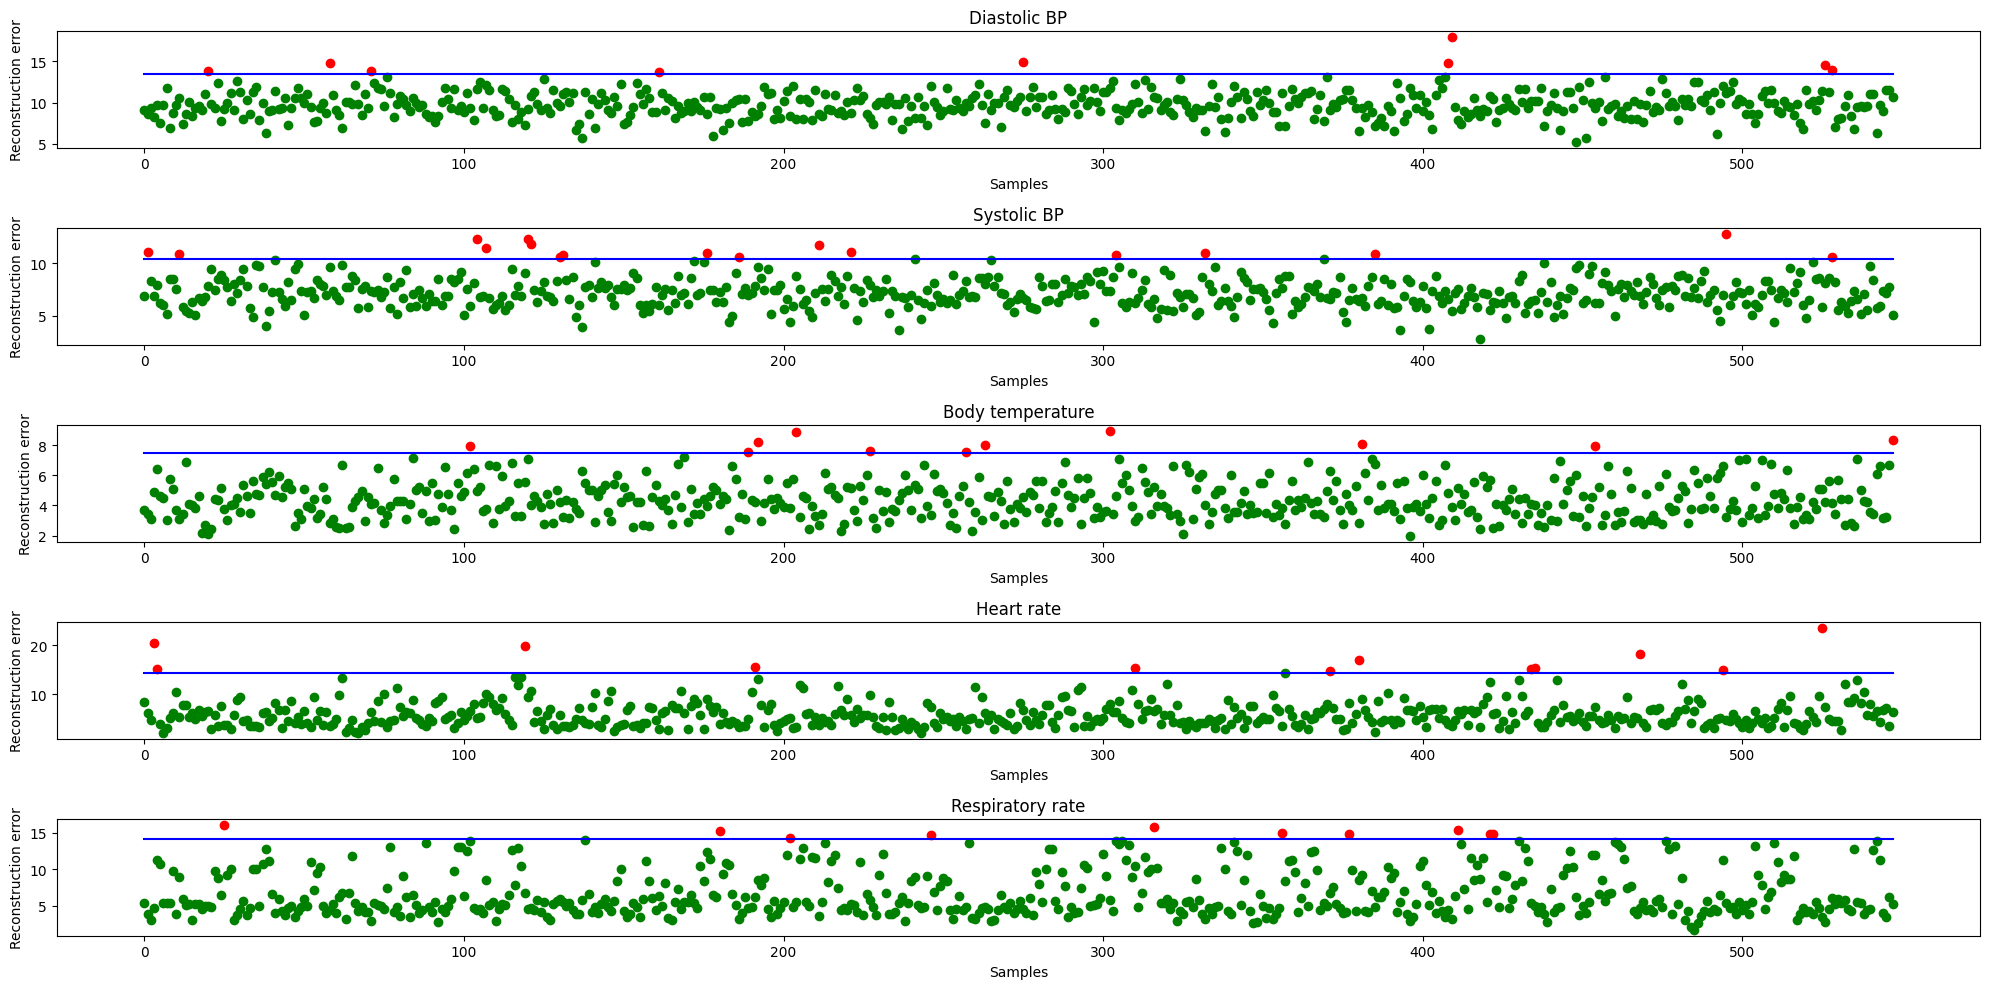
\includegraphics[width=\linewidth]{imgs/feature_test_err.png}}
	\caption{Anomalies in testing data}
	\label{fig:feature_test_data}
\end{figure}


\begin{figure}[H]
	\centering
	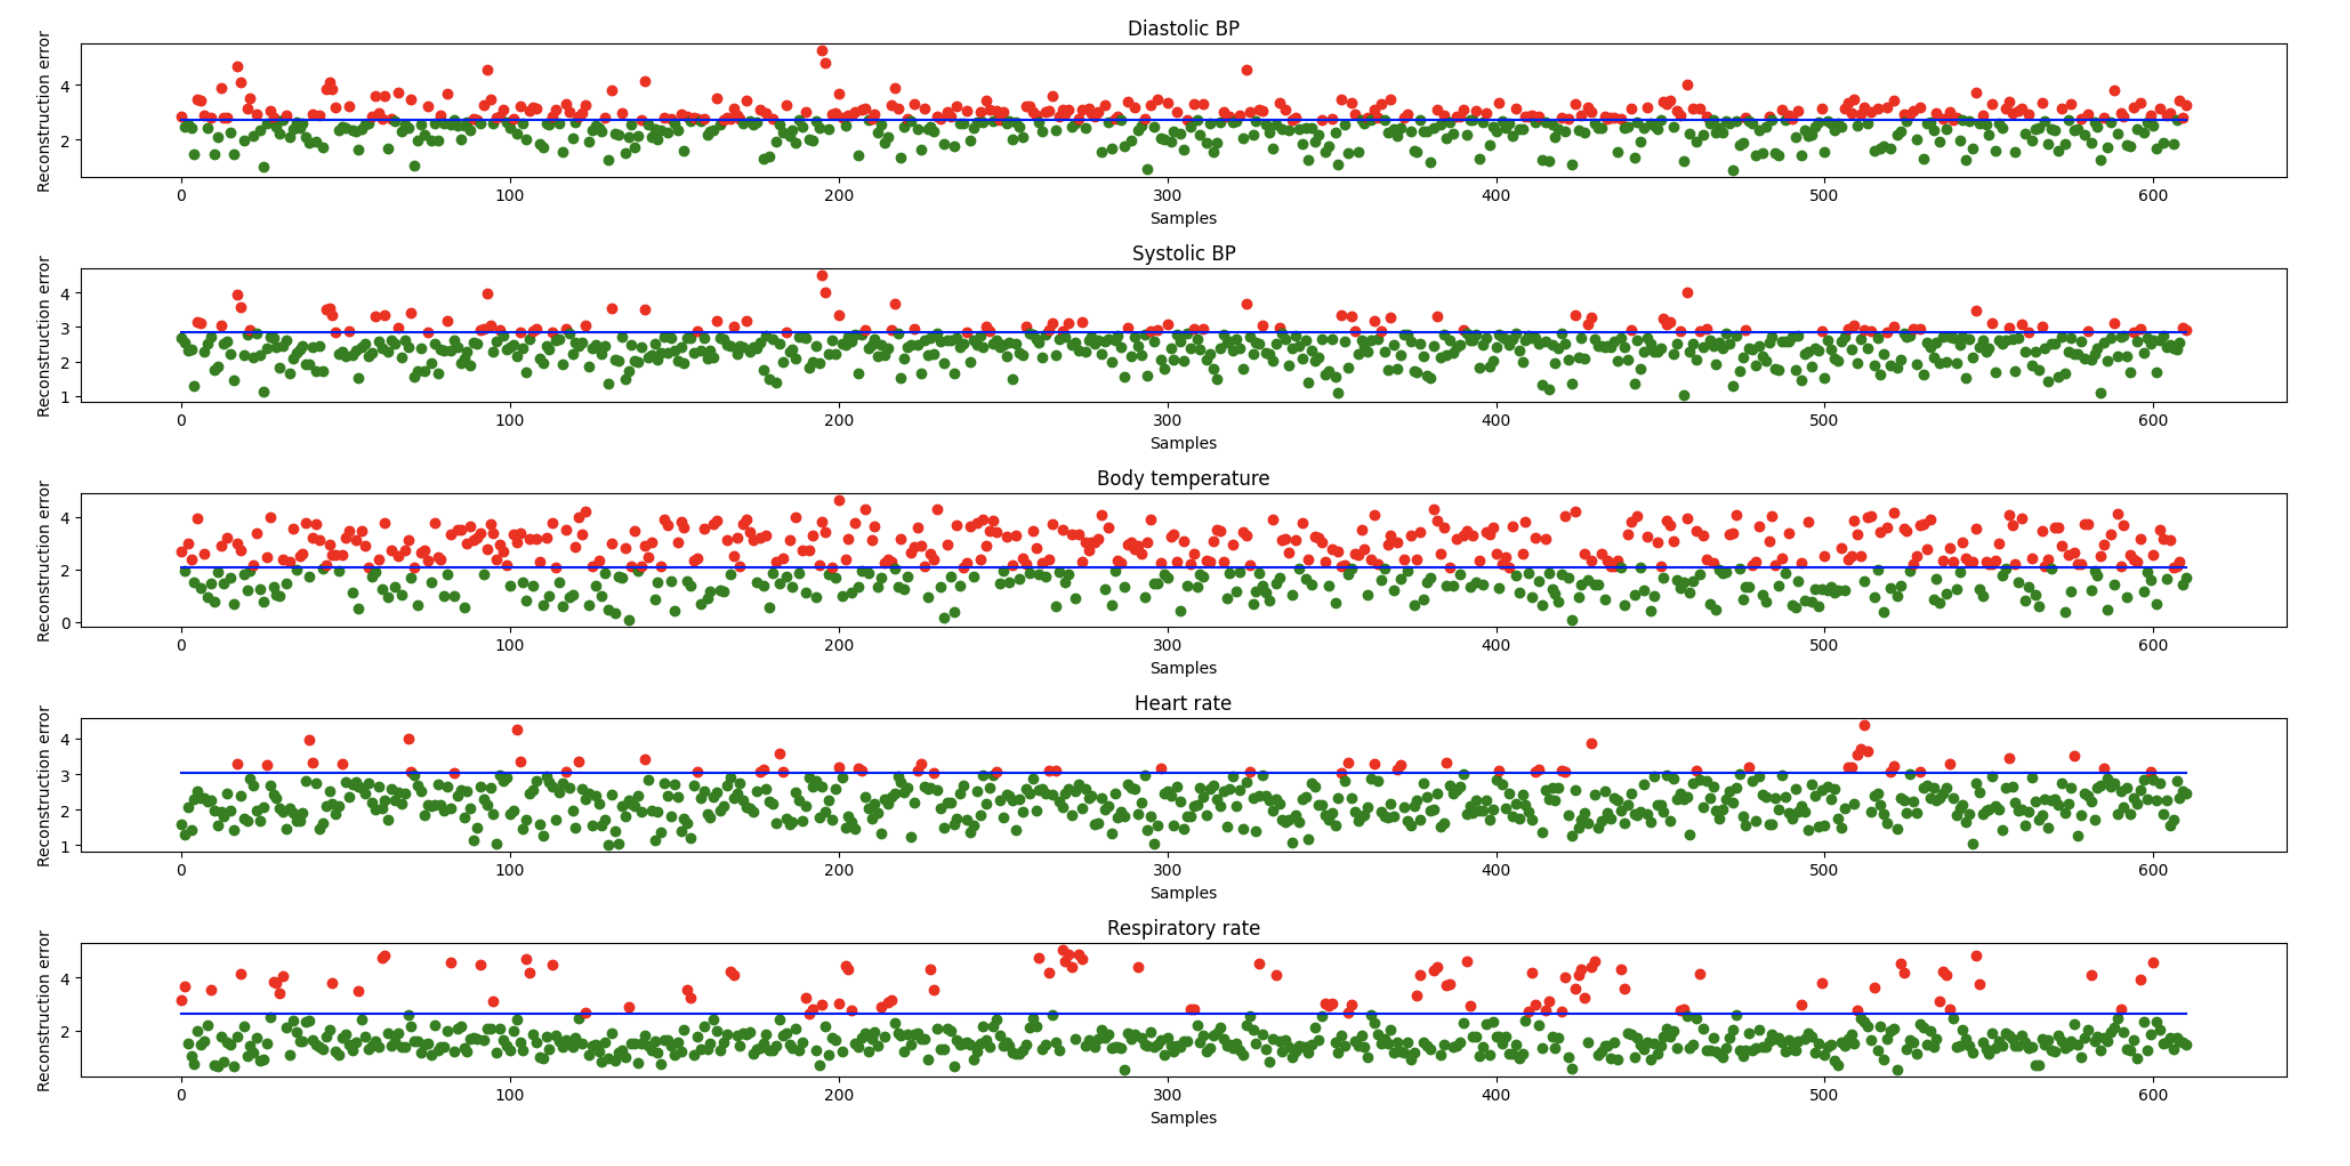
\includegraphics[width=\linewidth]{imgs/feature_asa3_err.png}
	\caption{Anomalies in data with ASA == 3}
	\label{fig:feature_asa3_data}
\end{figure}


An example of anomaly is shown in figure \ref{fig:anomaly}.


\begin{figure}[H]
	\centering
	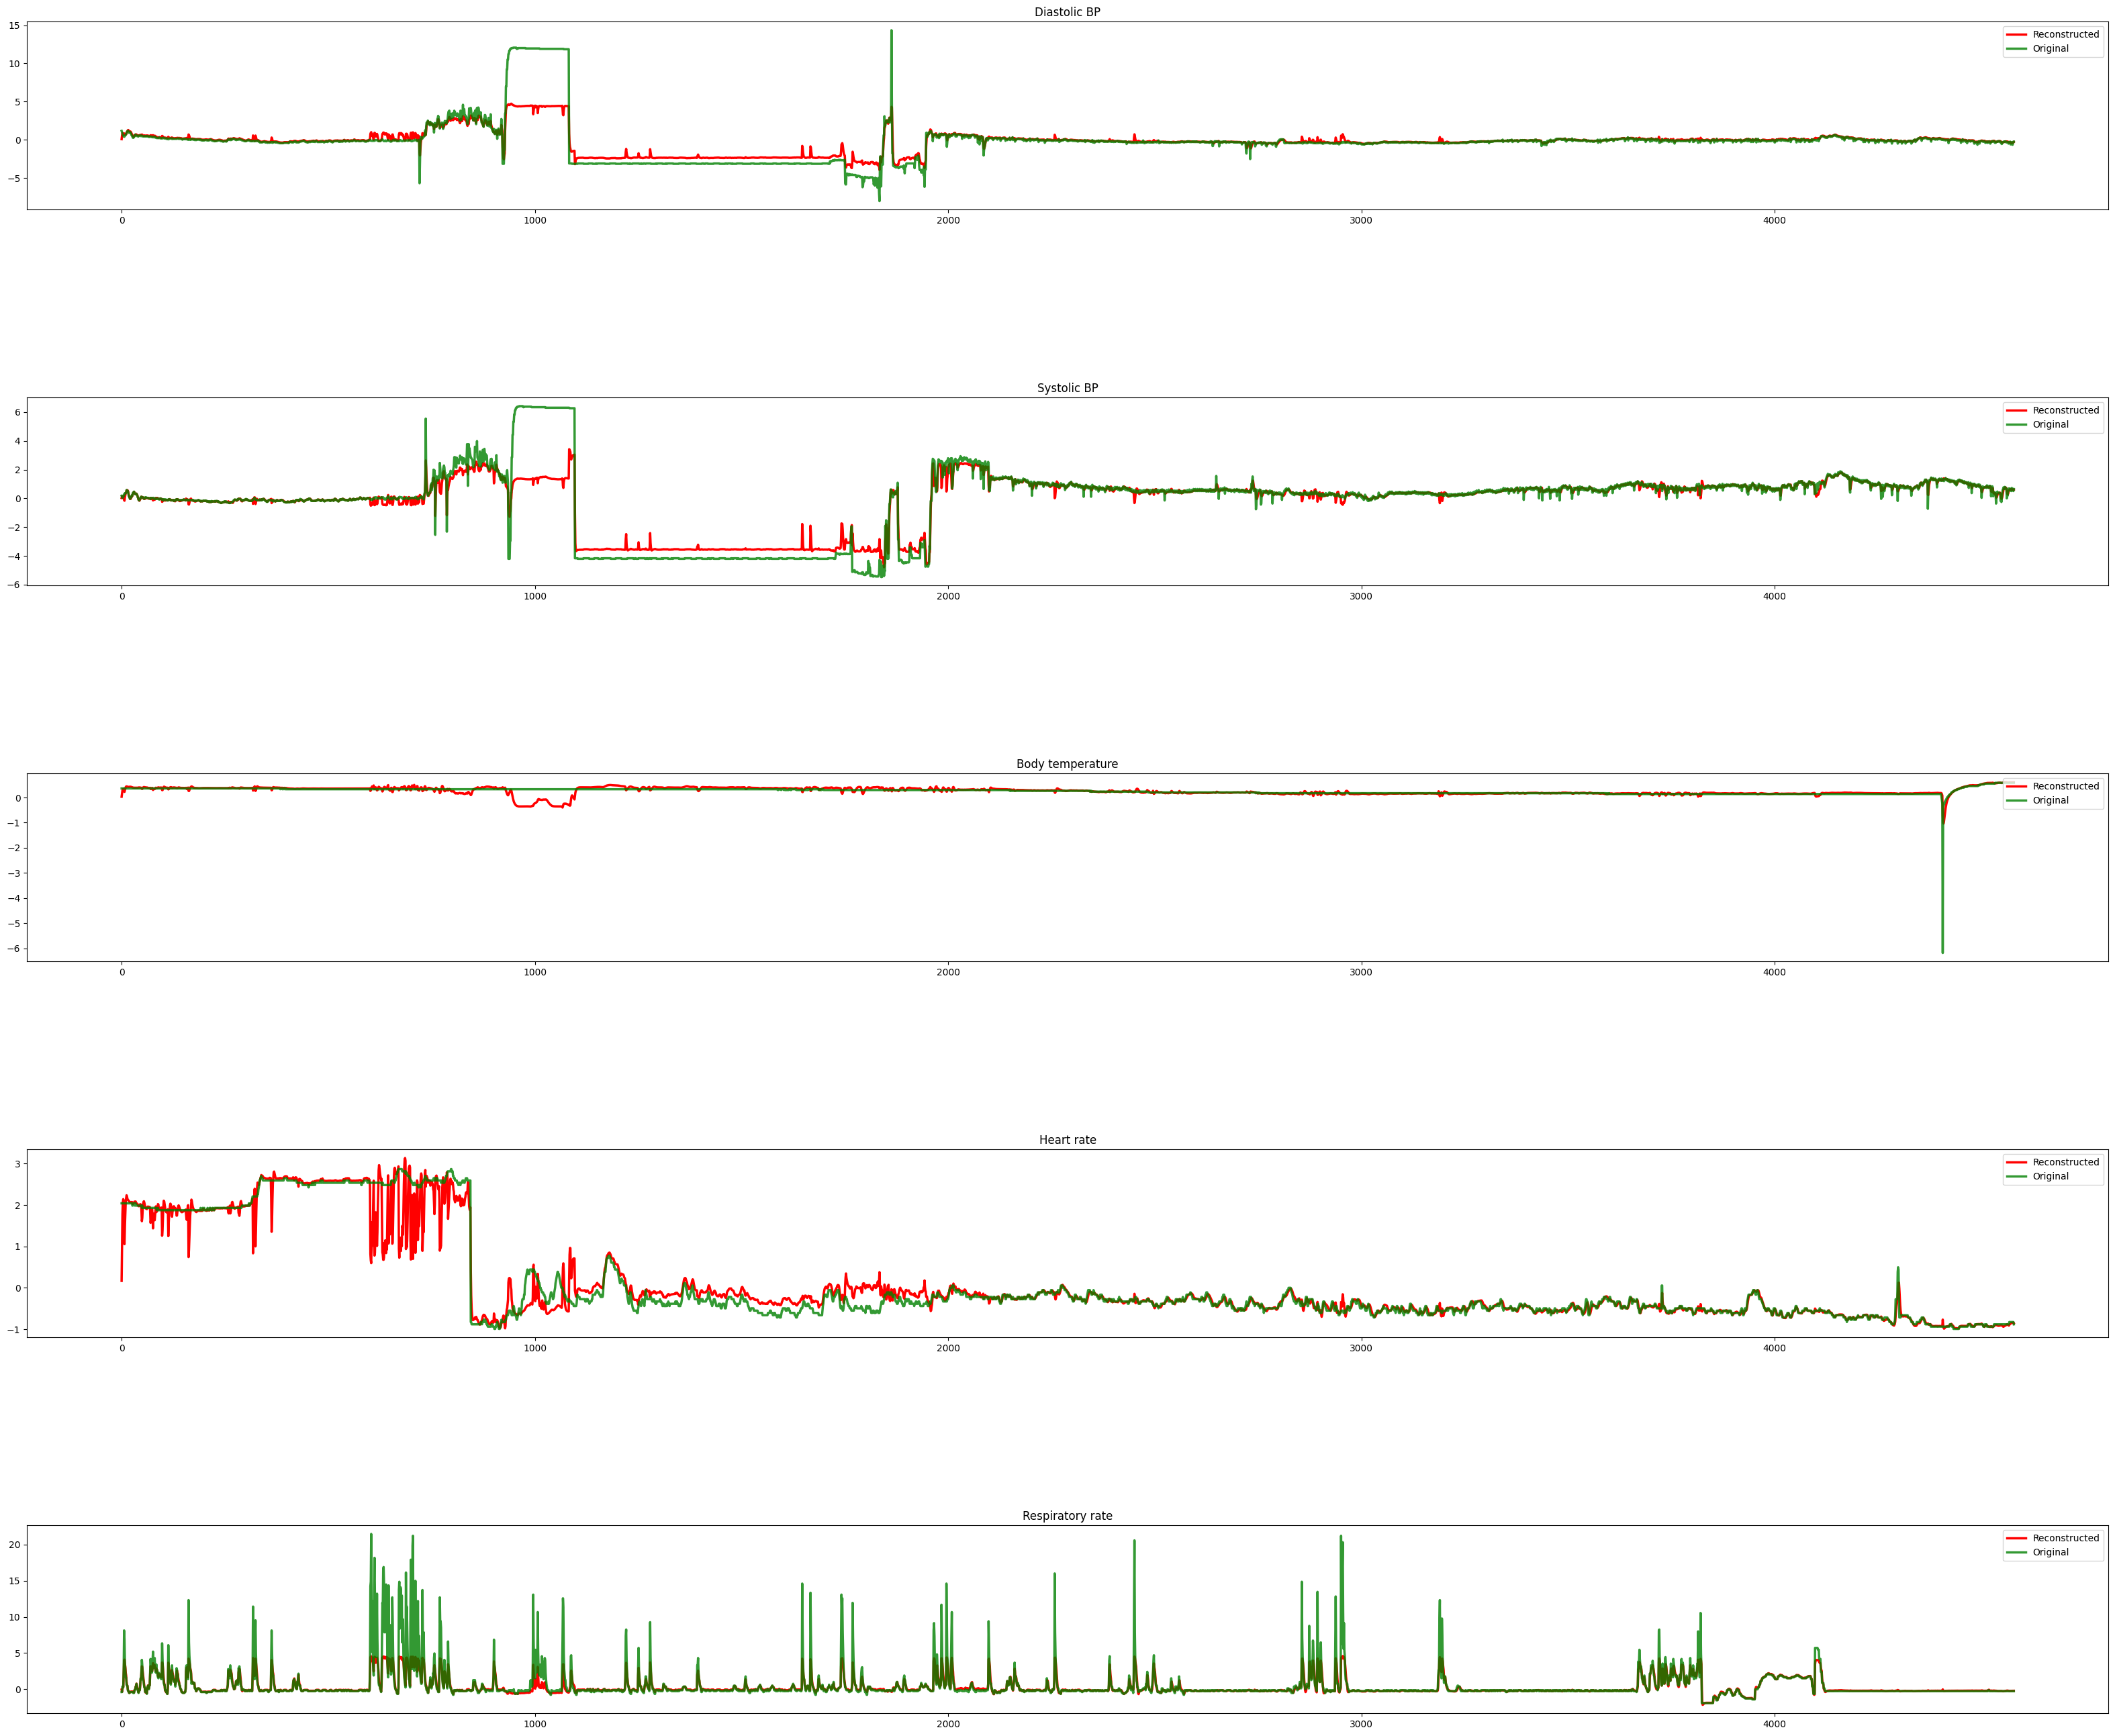
\includegraphics[width=\linewidth]{imgs/test_anomaly.png} 
	\caption{Anomaly in test data}
	\label{fig:anomaly}
\end{figure}



\section{Ethical implications}
		\label{ethics}

As the research in the e-health domain develops, a focus on the ethical implications is needed. As highlighted by Floridi, \cite{floridi2022etica} the explainability is a core ethical principle on which AI-enabled systems must be designed and developed in order to provide useful information about their processes and results. A sufficient, explicable process makes it possible to track the responsibilities and identify fallacies in an AI-enabled system. This requirement becomes crucial when such systems are employed in the health domain, since it is important to provide reliable information and verifiable processes. In the case of autoencoders where such properties are partially or merely satisfying, it's necessary to verify carefully their results before taking decisions, thus avoiding what Floridi calls "recycling of actions" i.e., acting as a computer suggests, only because we trust the results and how they are obtained.
Lastly, the nature and quality of the data used to train AI systems play a central role in their behavior and decision-making. This is why autoencoders like the one developed in this work, which is trained on surgical patient data, should be used to identify anomalies in the very same context where training data is collected since it could be misleading in other circumstances.


\section{Further developments}

The normal data can be bundled with the training set to expand it. By doing so, it is possible to detect concept drifts and adapt the threshold by running the algorithm \ref{threshold} on such new data.
Other techniques for anomaly detection could be applied to the very same dataset configuration in order to compare the results obtained from the autoencoder.
It is also possible to compare normalization schemes and see how they behave.
		
\nocite{*}
\printbibliography
		
		
	\end{multicols*}
	
\end{document}





